\documentclass{article}
\usepackage{graphicx} % Required for inserting images
\usepackage{parskip}
\usepackage{amsmath}
\usepackage{amssymb}
\usepackage{enumitem}
\usepackage{nicematrix}

\usepackage{hyperref}
\pdfstringdefDisableCommands{\def\eqref#1{(\ref{#1})}}

\usepackage{tikz}
\usetikzlibrary{positioning, arrows.meta}

\usepackage{biblatex}
\addbibresource{ref.bib}

\title{\textbf{Calculating error probabilities of group sequential clinical trials via a Markov process}}
\author{Mazin Abdelghany, MD, MS}
\date{May 2026}

\begin{document}

\maketitle
%
\section{Introduction}
%
Sequential clinical designs evaluate data as it is collected, and further sampling is stopped in accordance with a pre-defined stopping rule as soon as significant results are observed.

Interim analyses are performed at prespecified time points during trial conduct. These analyses allow for the option to stop the trial either for (1) futility if the results suggest that the treatment is unlikely to be efficacious, or (2) efficacy if the results suggest that the treatment differs substantially from control. 

Group sequential designs are multistage trials in which equal numbers of patients, $n$, are recruited at each stage. A trial design is specified by upper and lower boundaries at each stage. Consider a group-sequential design with $K$ total stages. The trial design $D$ will define upper and lower boundaries for each stage
%
\begin{equation}
    D = \{u_1, \ell_1, \dots,u_K,\ell_K\}
\end{equation}
%
At the $k$th analysis, a test statistic $Z_k$ is calculated using the patients recruited thus far. If $Z_k$ is between the boundaries for that stage, the trial continues. Otherwise, the trial is stopped either for futility or efficacy. The test statistics at each interim analysis $k$ (where $k = 1, 2,\dots, K$) form a multivariate normal distribution. Transitions from stage $k-1$ to stage $k$ are independent of previous stages (i.e., $k-2,k-3,\dots,1$). Formally,
%
\begin{equation}
    \Pr(Z_{k}\mid Z_{k-1} = z_{k-1}) = \Pr(Z_k \mid Z_{k-1} = z_{k-1}, Z_{k-2} = z_{k-2}, \dots, Z_1=z_1)
\end{equation}
%
We see that this is the definition of the Markov property. Taking advantage of this property allows us to solve one-dimensional integrals propagated across a transition probability matrix rather than multiple computationally expensive $\{1, 2, \dots, K-1, K\}$-dimensional multivariate normal integrals. The code in \texttt{pyGroupSequentialDesigns/simulate.py} does exactly that.
%
\section{Underlying stochastic process}
%
Let $Z_k$ be the standard normal test statistic calculated at interim analysis $k$. $Z_k$ has mean $\mu_k$, which is conditional on the assumed hypothesis (null or alternative) and dependent on the assumed variance.

The test statistics $Z_k$ and $Z_{(k-1)}$ follow a joint multivariate normal distribution
%
\begin{equation} \label{eq:joint_mvn}
    \begin{pmatrix}
        Z_{k-1} \\
        Z_k
    \end{pmatrix} \sim \mathcal{N}(\mathbf{\mu}, \mathbf{\Sigma}) = \mathcal{N}\left( \begin{bmatrix}
        \mu_{k-1}\\
        \mu_k
    \end{bmatrix}, \begin{bmatrix}
        \Sigma_{(k-1\mid k-1)} & \Sigma_{(k-1\mid k)} \\
        \Sigma_{(k\mid k-1)} & \Sigma_{(k\mid k)}
    \end{bmatrix} \right)
\end{equation}
%
Once we have realized a value for the random variable $Z_{k-1}=z_{k-1}$, we can use the conditional distributions for the mean and covariance of the multivariate normal to calculate the expected value of $Z_k$:
%
\begin{equation} \label{eq:cond_dist_zk}
    Z_{k}\mid Z_{(k-1)} \sim \mathcal{N}(\mu_{(k \mid k-1)},\Sigma_{(k\mid k-1)})
\end{equation}
%
where
\begin{align}
    \mu_{(k \mid k-1)} &= \mu_k + \Sigma_{(k \mid k-1)}\Sigma_{(k-1\mid k-1)}^{-1}(z_{k-1} - \mu_{k-1}) \label{eq:cond_mean} \\
    \Sigma_{(k\mid k-1)} &= \Sigma_{(k\mid k)} - \Sigma_{(k \mid k-1)}\Sigma_{(k-1\mid k-1)}^{-1}\Sigma_{(k-1\mid  k)} \label{eq:cond_covar}
\end{align}
%
As we are only going forward one stage per calculation, the above Eqs. \eqref{eq:cond_mean} and \eqref{eq:cond_covar} can be simplified. First, note that all of the elements of the covariance matrix, $\mathbf{\Sigma}$ in Eq. (\ref{eq:joint_mvn}), are scalars. Second, all covariances between a stage and itself (e.g., $\Sigma_{(k\mid k)}$) are equal to 1. Third, in the case of group sequential designs, $\Sigma_{(k \mid k-1)}=\Sigma_{(k-1\mid  k)}$. Thus,
%
\begin{align}
    \mu_{(k \mid k-1)} &= \mu_k + \Sigma_{(k \mid k-1)}(z_{k-1} - \mu_{k-1}) \label{eq:cond_mean_for_calc} \\
    \Sigma_{(k\mid k-1)} &= 1 - \Sigma_{(k \mid k-1)}^2 
\end{align}
%
If the covariance is $\Sigma_{(k\mid k-1)}$---and recalling that all elements of $\mathbf{\Sigma}$ are scalars in this case---then the standard deviation is simply:
%
\begin{equation}
    \sigma_{k\mid k-1}=\sqrt{1- \Sigma_{k\mid k-1}^2} \label{eq:cond_std_for_calc}
\end{equation}
%
Lastly, note that 
\begin{equation} \label{eq:cov_information}
    \mathrm{Cov}(Z_{k-1}, Z_k) = \Sigma_{k\mid k-1} = \sqrt{I_{k-1}/I_k},
\end{equation}
%
where $I$ is the information at each stage.
%
\section{Probabilities for Stage 1}
%
Calculating the stopping probabilities for Stage 1 are straightforward. The first realization of the test statistic $Z_1=z_1$ has a probability of crossing the defined upper boundary $u_1$ under hypothesis $H\in\{0,1\}$ where $H=0$ is the null hypothesis and $H=1$ is the alternative hypothesis of
\begin{equation}
    \Pr(Z_1 > u_1)=\int_{u_1}^\infty \phi\left(u_1-\mu_1^{(H)}\right)\,dz=1-\Phi\left(u_1-\mu_1^{(H)}\right)
\end{equation}
%
where $\phi(x)$ is the probability density function of the standard normal distribution and $\Phi(x)$ is the cumulative distribution function of the standard normal distribution. This is the probability of stopping for \textbf{efficacy} at the first stage.

Note that $u_1$ is standardized by the mean at the first stage under the hypothesis in question. Let $\mu_{k}^{(H)}$ be the mean under the  hypothesis in question at stage $k$, and given assumed values for the parameter of interest $\theta_H$ under the null and alternative hypotheses, the standardized means for each stage are calculated by
%
\begin{equation} \label{eq:mu_k}
    \mathbb{E}[Z_k]=\mu_k^{(H)}=\theta_H\sqrt{I_k}
\end{equation}
%
Similarly, the first realization of the test statistic $Z_1=z_1$ has probability of crossing the defined lower boundary $\ell_1$ of
%
\begin{equation}
    \Pr(Z_1 \le \ell_1)=\int_{-\infty}^{\ell_1} \phi\left(\ell_1-\mu_1^{(H)}\right)\,dz=\Phi\left(\ell_1-\mu_1^{(H)}\right)
\end{equation}
%
This is the probability of stopping for \textbf{futility} at the first stage.
\section{Probabilities for Stages 2 to \texorpdfstring{$K$}{}}
%
In order to calculate the probability of stopping under the hypothesis in question for stages 2 through $K$, multidimensional integrals must be solved. Generally, for $k$ stages, the following integral calculates the probability of stopping for \textbf{futility} under hypothesis $H$ at stage $k$,
%
\begin{equation} \label{eq:fut_integral}
    \Pr\left(\mathrm{Fut}_k^{(H)}\right)=\int_{\ell_1}^{u_1} \cdots \int_{\ell_{k-1}}^{u_{k-1}}\int_{-\infty}^{\ell_k} f(z_1,\dots,z_k\mid\theta_H)\,dz_k,dz_{k-1},\dots,dz_1
\end{equation}
%
and for \textbf{efficacy} under the hypothesis $H$ at stage $k$,
%
\begin{equation} \label{eq:eff_integral}
    \Pr\left(\mathrm{Eff}_k^{(H)}\right)=\int_{\ell_1}^{u_1} \cdots \int_{\ell_{k-1}}^{u_{k-1}}\int_{u_k}^{\infty} f(z_1,\dots,z_k\mid\theta_H)\,dz_k,dz_{k-1},\dots,dz_1
\end{equation}
%
As the number of stages increases, complexity of these multidimensional integrals increases exponentially. For example, to calculate relevant statistics (e.g., type I and II error), a 3-stage trial requires solving a 1-, 2- and 3-dimensional integrals for futility and efficacy under both the null and alternative.

In order to simplify these multidimensional integrals into one-dimensional integrals, we first introduce the basics of Markov processes and the Chapman-Kolmogorov equation (CKE). 

Our Markov process can be illustrated as follows:
\vspace{2mm}
\begin{center}
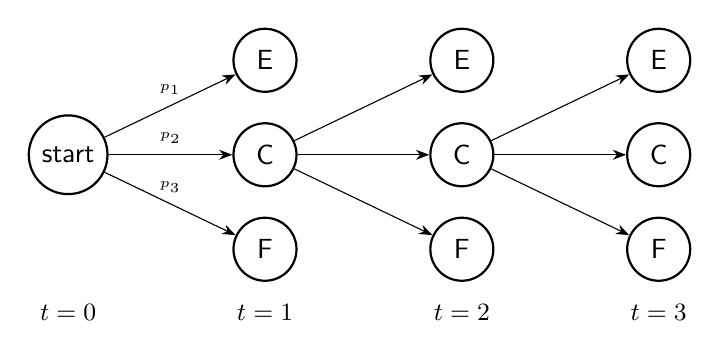
\begin{tikzpicture}[
    ->, >=Stealth,
    state/.style={circle, draw, minimum size=0.8cm, font=\sffamily, thick},
    time_label/.style={font=\small\bfseries, yshift=-0.5cm},
    label_style/.style={midway, above, yshift=3pt, font=\tiny, fill=white, inner sep=1pt}
]

    % Define t=0 (Initial Node)
    \node[state] (C0) at (0, 1.2) {start};
    \node[time_label] at (0, -0.3) {$t=0$};

    % Define columns t=1, 2, 3
    \foreach \t in {1, 2, 3} {
        \node[state] (E\t) at (\t*2.5, 2.4) {E};
        \node[state] (C\t) at (\t*2.5, 1.2) {C};
        \node[state] (F\t) at (\t*2.5, 0.0) {F};
        
        \node[time_label] at (\t*2.5, -0.3) {$t=\t$};
    }

    % Transitions from t=0 to t=1
    \draw[thin] (C0) -- (E1) node[label_style] {$p_1$};
    \draw[thin] (C0) -- (C1) node[label_style] {$p_2$};
    \draw[thin] (C0) -- (F1) node[label_style] {$p_3$};

    % Transitions from C nodes only for subsequent steps
    \foreach \source [evaluate=\source as \next using int(\source+1)] in {1, 2} {
        \draw[thin] (C\source) -- (E\next);
        \draw[thin] (C\source) -- (C\next);
        \draw[thin] (C\source) -- (F\next);
    }

\end{tikzpicture}
\end{center}
%
with its state space $\mathcal{S}=\{E, C,F\}$.

The trial starts at the first node at time 0. After data are collected, the trial may continue (node C), stop for efficacy (node E), or stop for futility (node F) and the probabilities of each edge are calculated as discussed above. E and F nodes do not have edges as the trial has stopped and cannot progress to the next stage.

Let us consider a \textbf{discrete} path that goes from stage $i$ to stage $j$ through stage $k$. In other words, we have
%
\[i\to k \to  j.\]
%
Further, let us assume that it takes $m$ stages to go from stage $i$ to $k$ and another $n$ stages to go from stage $k$ to $j$. We can depict this as
%
\[
i\xrightarrow{m \text{ steps }}k\xrightarrow{n \text{ steps }}j
\]
%
If we are interested in calculating the probability of moving from stage $i$ to stage $j$, $\Pr_{ij}^{(n+m)}$, we must consider all of the probabilities of the paths that take us from $i$ to $j$ through $k$, that is $\Pr_{ik}^{(m)}$ and $\Pr_{kj}^{(n)}$, within the state space $\mathcal{S}$.

This probability is given by the CKE for the discrete case:
%
\begin{align}
    \underbrace{\Pr\nolimits_{ij}^{(n+m)}}_{\text{where we're going}} &= \sum_{k\in\mathcal{S}} \Pr\nolimits_{ik}^{(m)} \Pr\nolimits_{kj}^{(n)}\\
    &=\underbrace{\sum_{k\in\mathcal{S}}}_{\text{all possible paths}} \underbrace{ \Pr(X_m=k\mid X_0=i) }_{\text{where we've been}} \underbrace{\Pr(X_{n+m} = j \mid X_m=k)}_{\text{one possible path to get there}}
\end{align}
%
Plainly, to calculate the probability of the stage to which we are going ($j$), we multiply the probability of going from the start to the current stage ($k$) by one possible way of getting from stage $k$ to stage $j$. In order to get the total probability, we must sum this multiplication over all of the possible ways of getting from $k$ to $j$.

Analogously, for our group sequential trials, we can write
%
\begin{equation} \label{eq:cke_brackets}
    \underbrace{f_k(z_k\mid\theta)}_{\text{where we're going }} = \underbrace{\int_{z_{k-1}\in\mathcal{S}}}_{\text{ all possible paths }} \underbrace{f_{k-1}(z_{k-1}\mid\theta)}_{\text{ where we've been }}\,\underbrace{g_k(z_{k-1},z_k\mid \theta)}_{\text{ one possible path }}\,dz_{k-1}
\end{equation}
%
where $z_{k-1}$ is one possible state within the previous continuation region, i.e., $y\in(\ell_{k-1},u_{k-1})$. Importantly, $f_k(z_k)$ is the \textbf{joint probability subdensity function} for continuation to Stage $k$.

The integral in Eq. \eqref{eq:cke_brackets} is the same as Eq. (8.6) in \textcite{jennison1999group} ($f$ and $g$ from the original are exchanged for clarity to match our analysis thus far):
\begin{equation} \label{eq:cke_jennison}
    f_k(z_k\mid\theta)=\int_{\mathcal{C}_{k-1}} f_{k-1}(z_{k-1}\mid\theta)\,g_k(z_{k-1},z_k\mid\theta)\,dz_{k-1}
\end{equation}
%
for $k=2,\dots,K$, where 
\begin{equation} \label{eq:jennison_g}
    g_k(z_{k-1},z_k\mid\theta)=\frac{\sqrt{I_k}}{\sqrt{\Delta_k}}\,\phi\left(\frac{z_k\sqrt{I_k}-z_{k-1}\sqrt{I_{k-1}}-\Delta_k\theta}{\sqrt{\Delta_k}}\right)
\end{equation}
%
and where $\mathcal{C}_{k-1}$ is the continuation region equivalent to our state space and 
%
\begin{equation} \label{eq:delta_k}
    \Delta_k=I_k-I_{k-1}
\end{equation}
%
Note that $f_{k-1}(y)$ is not a standard probability density. In Chapter 19, \textcite{jennison1999group} explain that $f_k(z_k\mid\theta)$ for $k=1,\dots,K$ represent \textbf{subdensities} of $\{Z_1,\dots,Z_k\}$ with their integrals all evaluating to less than 1 for $k>1$ because of early stopping at stages $1,\dots,k-1$.

$g_k(z_{k-1},z_k\mid \theta)$ calculates the \textit{conditional} probability \textbf{density} of moving from stage $k-1$ to $k$ for a certain realization of $Z_k$. This probability density of the stepping from a point at Stage $k-1$ to a point at Stage $k$ is normally distributed with mean and covariance related to the hypothesis in question and given by Eqs. \eqref{eq:cond_mean_for_calc} and \eqref{eq:cond_std_for_calc}, respectively. Combining Eq. \eqref{eq:cond_dist_zk} with Eqs. \eqref{eq:cond_mean_for_calc} and \eqref{eq:cond_std_for_calc}, we write:
%
\begin{equation}
    Z_{k}\mid Z_{(k-1)} \sim \mathcal{N}\left(\mu_k + \Sigma_{(k \mid k-1)}(z_{k-1} - \mu_{k-1}), 1 - \Sigma_{(k \mid k-1)}^2\right)
\end{equation}
%
Using this fact, we can expand $g_k(z_{k-1},z_k\mid \theta)$, applying the same standardization that was performed for the calculation of the probabilities for Stage 1. In this case, the denominator is not 1 (as it is in Stage 1) because there is a covariance between stages that needs to be taken into account.
%
\begin{equation} \label{eq:g_implemented}
    g_k(z_{k-1},z_k\mid \theta) = \frac{1}{\sqrt{1 - \Sigma_{(k \mid k-1)}^2}}\,\phi\left(\frac{z_k-\left[\mu_k + \Sigma_{(k \mid k-1)}(z_{k-1} - \mu_{k-1})\right]}{\sqrt{1 - \Sigma_{(k \mid k-1)}^2}}\right)
\end{equation}
% space below purposeful 

With some straightforward algebra, we can show that Eq. \eqref{eq:jennison_g} is equal to Eq. \eqref{eq:g_implemented}, see Appendix \ref{appendix:a}. 

The joint probability subdensity function in Eq. \eqref{eq:cke_jennison} can be integrated---marginalizing over $z_{k-1}$---in order to calculate the stopping probabilities for futility and efficacy as in Eqs. \eqref{eq:fut_integral} and \eqref{eq:eff_integral}, respectively. Specifically,
%
\begin{align}
    \Pr(\mathrm{Fut}_k) &= \int_{-\infty}^{\ell_{k}} f_k(z_k\mid\theta)\,dz_k\\
    &=\int_{\ell_{k-1}}^{u_{k-1}}\int_{-\infty}^{\ell_{k}} f_{k-1}(z_{k-1}\mid\theta)\,g_k(z_{k-1},z_k\mid\theta)\,dz_k\, dz_{k-1} \\
    &= \int_{\ell_{k-1}}^{u_{k-1}}f_{k-1}(z_{k-1}\mid\theta) \int_{-\infty}^{\ell_{k}} \,g_k(z_{k-1},z_k\mid\theta)\,dz_k \,dz_{k-1}\label{eq:double_int} \\
    &= \int_{\ell_{k-1}}^{u_{k-1}}f_{k-1}(z_{k-1}\mid\theta)\cdot \nonumber \\
    &\qquad\qquad \Phi\left( \frac{l_k -\left[\mu_k + \Sigma_{(k \mid k-1)}(z_{k-1} - \mu_{k-1})\right]}{\sqrt{1 - \Sigma_{(k \mid k-1)}^2}} \right) dz_{k-1} \label{eq:final_fut}
\end{align}
%
Going from Eq. \eqref{eq:double_int} to Eq. \eqref{eq:final_fut} uses the definition of the conditional multivariate normal mean and standard deviation and the definition of the normal cumulative distribution function.

A similar procedure can be used to derive the probability of stopping for efficacy:
\begin{align} \label{eq:final_eff}
    \Pr(\text{Eff}_k) &= \int_{l_{k-1}}^{u_{k-1}} f_{k-1}(z_{k-1}\mid\theta) \cdot \nonumber \\
    &\qquad\qquad\left[ 1 - \Phi\left( \frac{u_k -\left[\mu_k + \Sigma_{(k \mid k-1)}(z_{k-1} - \mu_{k-1})\right]}{\sqrt{1 - \Sigma_{(k \mid k-1)}^2}} \right) \right] dz_{k-1}
\end{align}
%
\section{Computing probabilities with quadrature}
%
In order to compute Eqs. \eqref{eq:final_fut} and \eqref{eq:final_eff} numerically, we need to discretize the integral into a summation. Again, borrowing an idea from Markov processes, we can generate a sufficiently dense transition probability matrix $\mathbf{T}_k$ that can then be used to calculate the probabilities using quadrature.

First, the continuation regions for stage $k-1$ and stage $k$ are partitioned into a set number of grid points $G$ where $\Delta z =(u_k-\ell_k)/G$. The transition probability densities (the elements of $\mathbf{T}_k$) from one possible grid point realization going to the next ($Z_{k-1}=z_{k-1} \to Z_k=z_k$) are then calculated according to Eq. \eqref{eq:g_implemented}.
%
\begin{center}
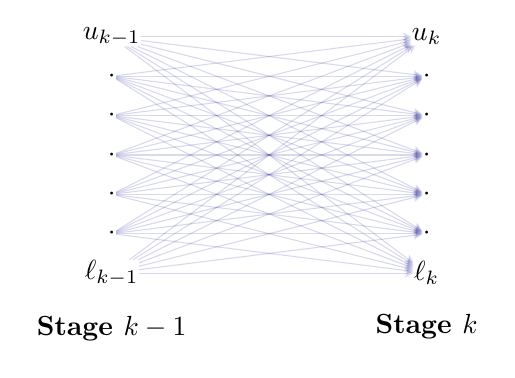
\begin{tikzpicture}[
    node distance = 1.5cm,
    % Style for the invisible nodes that hold the dots/labels
    dot/.style = {inner sep=0pt, minimum size=0pt},
    % Style for the arrows: thin and semi-transparent for the criss-cross effect
    arrow/.style = {->, >=stealth, thin, opacity=0.15, blue!50!black} 
]

    % --- STAGE k-1 (Left Column) ---
    \node[dot] (L1) at (0, 3) {$u_{k-1}$};
    \node[dot] (L2) at (0, 2.5) {$\cdot$};
    \node[dot] (L3) at (0, 2) {$\cdot$};
    \node[dot] (L4) at (0, 1.5) {$\cdot$};
    \node[dot] (L5) at (0, 1) {$\cdot$};
    \node[dot] (L6) at (0, 0.5) {$\cdot$};
    \node[dot] (L7) at (0, 0) {$\ell_{k-1}$};
    
    \node[below=0.25cm of L7, font=\bfseries] {Stage $k-1$};

    % --- STAGE k (Right Column) ---
    \node[dot] (R1) at (4, 3) {$u_k$};
    \node[dot] (R2) at (4, 2.5) {$\cdot$};
    \node[dot] (R3) at (4, 2) {$\cdot$};
    \node[dot] (R4) at (4, 1.5) {$\cdot$};
    \node[dot] (R5) at (4, 1) {$\cdot$};
    \node[dot] (R6) at (4, 0.5) {$\cdot$};
    \node[dot] (R7) at (4, 0) {$\ell_k$};
    
    \node[below=0.25cm of R7, font=\bfseries] {Stage $k$};

    % --- ALL-TO-ALL CRISS-CROSS ARROWS ---
    % This nested loop connects every node in column L to every node in column R
    \foreach \i in {1,...,7} {
        \foreach \j in {1,...,7} {
            \draw[arrow] (L\i) -- (R\j);
        }
    }

\end{tikzpicture}
\end{center}

Each arrow above represents a probability of going from one realization of $z$ at Stage $k-1$ to another realization of $z$ at Stage $k$ and is represented by a single value in $\mathbf{T}_k$. 

In an overly simplified example, assume that $G=5$, then $\mathbf{T}_k$ is
%
\[ 
\begin{NiceArray}{c@{\hspace{1.25em}}ccccc c}[margin] 
         & \ell_{k-1} &  &  & \Cdots & u_{k-1} & k-1 \\[5px] 
  \ell_k & a_{11} & a_{12} & a_{13} & a_{14} & a_{15} \\ 
  \Vdots & a_{21} & a_{22} & a_{23} & a_{24} & a_{25} \\[5px]
         & a_{31} & a_{32} & a_{33} & a_{34} & a_{35} \\[5px]
         & a_{41} & a_{42} & a_{43} & a_{44} & a_{45} \\[5px]
  u_k    & a_{51} & a_{52} & a_{53} & a_{54} & a_{55} \\[5px] 
  k 
\CodeAfter 
    \SubMatrix[{2-1}{6-1}] % Vertical labels on the left
    \SubMatrix[{1-2}{1-6}] % Horizontal labels on the top
    \SubMatrix[{2-2}{6-6}] % Main 5x5 matrix
\end{NiceArray} 
\]
%
The row vector above the matrix represents the discretized possible nodes for the continuation region of Stage $k-1$ (the ``where we've been vector"). The column vector to the left of the matrix represents the discretized possible nodes for Stage $k$ (the ``where we're going vector"). The values of the matrix $a_{ij}$ are the probability \textbf{density} values calculated using $g(z_{k-1},z_k\mid\theta)$ for the probability of moving from one point in the row vector to one point in the column vector. The finer the grid, the more accurate the probability density estimates. 

The algorithm to calculate the probabilities Eqs. \eqref{eq:final_fut} and \eqref{eq:final_eff} is as follows below. The arguments of the standard normal cumulative density function are left out for brevity. Note that we are abusing the notation of the integral operator by including vectors within in. In fact, integrals will be estimated numerically with the trapezoidal rule (see below).

\textbf{Stage 1:}
\begin{itemize}[label={--}]
    \item $\Pr(\mathrm{Eff_1})=1-\Phi$
    \item $\Pr(\mathrm{Fut_1})=\Phi$
\end{itemize}

\textbf{Stage 2:}
\begin{itemize}[label={--}]
    \item Calculate the density $f_{k-1}(z_{k-1}\mid\theta)$ from Eqs. \eqref{eq:final_fut} and \eqref{eq:final_eff}
        \begin{itemize}[label={\raisebox{0.25ex}{\scalebox{0.75}{\textbullet}}}]
            \item For Stage 2, this is $f_{1}(z_{1}\mid\theta)$
            \item Split the interval $(u_1,\ell_1)$ into $G$ grid points: $\mathbf{z}^{(1)}=\begin{bmatrix}
                z_1^{(1)},z_2^{(1)},\dots,z_G^{(1)}
            \end{bmatrix}$
            \item Condition this by the mean of the hypothesis in question ($\theta\sqrt{I}$)
            \item Calculate $f_1$ from Eq. \eqref{eq:cke_jennison}. Get a grid of densities by passing this standardized grid to the standard normal probability density function. Call this vector $\mathbf{d}_1$.
       \end{itemize}
    \item[] Eqs. \eqref{eq:final_fut} and \eqref{eq:final_eff}:
    \item $\Pr(\mathrm{Eff_2})=\int_{\ell_{1}}^{u_{1}} \mathbf{d}_1 \cdot(1-\Phi)\,dz_1$
    \item $\Pr(\mathrm{Fut_2})=\int_{\ell_{1}}^{u_{1}} \mathbf{d}_1 \cdot \Phi\,dz_1$
\end{itemize}

The first vector of densities $\mathbf{d}_1$ is not conditional on any stage before and therefore is not calculated using the matrix $\mathbf{T}_k$ described above.

\textbf{Stage 3:}
\begin{itemize}[label={--}]
    \item Calculate the density $f_{k-1}(z_{k-1}\mid\theta)$ from Eqs. \eqref{eq:final_fut} and \eqref{eq:final_eff}
    \begin{itemize}[label={\raisebox{0.25ex}{\scalebox{0.75}{\textbullet}}}]
            \item For Stage 3, this is $f_{2}(z_{2}\mid\theta)$
            \item Split the interval $(u_2,\ell_2)$ into $G$ grid points: $\mathbf{z}^{(2)}=\begin{bmatrix}
                z_1^{(2)},z_2^{(2)},\dots,z_G^{(2)}
            \end{bmatrix}$
            \item Generate the transition matrix $\mathbf{T}_2$. 
            \begin{itemize}[label={$\circ$}]
                \item For each value in $\mathbf{z}^{(1)}$ and $\mathbf{z}^{(2)}$,
                \item Standardize $\mathbf{z}^{(2)}$ by the conditional mean and conditional standard deviation of the hypothesis in question and the prior $z_1$ value (``where we've been"). This is the argument passed to $\phi(\cdot)$ in Eq. \eqref{eq:g_implemented}.
                \item Pass into the standard normal probability density function. This value is $\phi(\cdot)$ in Eq. \eqref{eq:g_implemented}.
            \end{itemize}
            \item Multiply $\mathbf{T}_2$, element-wise (operator $\odot$), by $\mathbf{d}_1$. This is the joint probability subdensity matrix that, integrated over $\mathcal{C}_{k-1}$, becomes density $f_2$ from Eq. \eqref{eq:cke_jennison}. Call this vector $\mathbf{d}_2$.
       \end{itemize}
    \item[] Eqs. \eqref{eq:final_fut} and \eqref{eq:final_eff}:
    \item $\Pr(\mathrm{Eff_3})=\int_{\ell_{2}}^{u_{2}} \mathbf{d}_2 \cdot(1-\Phi)\,dz_2$
    \item $\Pr(\mathrm{Fut_3})=\int_{\ell_{2}}^{u_{2}} \mathbf{d}_2 \cdot \Phi\,dz_2$
\end{itemize}

The process in Stage 3 is looped until stage $K-1$. This last loop generates $\mathbf{T}_{K-1}$, which is used to calculate $\mathbf{d}_{K-1}$ to estimate $\Pr(\mathrm{Eff_K})$ and $\Pr(\mathrm{Fut_K})$.
%
\subsection{Application of the trapezoidal rule}
%
In order to estimate the value of the integrals, we use the composite trapezoidal rule. The trapezoidal rule approximates the region under the graph of a function $f(x)$ over an interval $[a, b]$ as a trapezoid and calculating its area by noting that the region is made up of a rectangle with width $(a-b)$ and height $f(a)$ and triangle with the same width and height $f(a)-f(b)$.
\begin{align}
    \int_a^b f(x)\,dx &\approx (b-a)f(a)+ \frac{1}{2}(b-a)[f(b)-f(a)] \\
    &=(b-a)\left( f(a)+\frac{1}{2}f(b)-\frac{1}{2}f(a) \right)\\
    &=\frac{1}{2}(b-a)[f(a)+f(b)]
\end{align}
%
If $\{x_k\}$ is a partition of $[a,b]$ and $\Delta x_k=x_k-x_{k-1}$, then
\begin{equation}
    \int_a^b f(x)\,dx \approx \sum_{k=1}^N \frac{f(x_{k-1})+f(x_k)}{2} \Delta x_k
\end{equation}
%
If the spacing of the partition is regular and our partition is $\{x_0,\dots,x_N\}$, this can be further simplified to:
%
\begin{align} \label{eq:trap_rule}
    \int_a^b f(x)\,dx \approx \Delta x\left(\frac{f(x_0)+f(x_N)}{2} + \sum_{k=1}^{N-1}f(x_k)\right)
\end{align}
%
The argument for our integral is calculated by $\mathbf{d}_{k-1} \cdot \Phi$, and then the trapezoidal rule is applied exactly as shown in Eq. \eqref{eq:trap_rule}. To obtain the joint probability subdensity matrix, we multiply $\mathbf{T}_{k} \odot \mathbf{d}_{k-1}$. The integral matrix is then ``integrated" over $\mathcal{C}_{k-1}$ by finding its row sums, the summation in Eq. \eqref{eq:trap_rule}, and then multiplying by $\Delta z$. 

The final output is a vector---with the length of the number of stages of the trial---of futility and efficacy probabilities for the hypothesis in question.
%
\section{Error probabilities and expected sample size}
%
Once the loop calculates the individual probability vectors across all $K$ stages, the sums provide the statistical properties of interest.

Type I Error ($\alpha$) -- The total probability of crossing an efficacy bound at any stage under the null hypothesis ($\theta = \theta_0$):
%
\[
    \alpha = \sum_{k=1}^{K} P(\text{Eff}_k \mid \theta_0)
\]
$$$$
%
Power -- The total probability of crossing an efficacy bound at any stage under the alternative hypothesis ($\theta = \theta_1$):
%
\[
    \text{Power} = \sum_{k=1}^{K} P(\text{Eff}_k \mid \theta_1)
\]
%
Expected Sample Size (ESS) -- The average number of patients enrolled before the trial halts, calculated as the expected value under the assumption of a clinically relevant treatment effect $\delta=\theta_1-\theta_0$:
%
\begin{align}
    \mathbb{E}[N\mid\delta] &= \sum_{i=1}^k \big[i\cdot n\cdot\Pr(\text{trial stops after analysis }i\mid\delta)\big] \\
    &=\sum_{i=1}^k \Big( i\cdot n \cdot \big[ P(\text{Fut}_i \mid \delta) + P(\text{Eff}_i \mid \delta) \big] \Big)
\end{align}
%
where $n$ is the number of patients recruited per stage and is equal at each stage in the case of group sequential trials.
%
\section{Error analysis}
%
Two methods were assessed during error analysis---the trapezoidal rule, Simpson's rule, and the midpoint rule---and compared to the multivariate normal integration method utilized by \texttt{scipy}. 

Comparing results with the \texttt{scipy} integrator is difficult as it uses Monte Carlo simulation to estimate the integral. However, a clear pattern was noted in the analysis. The trapezoidal integration was consistently more accurate regardless of the number of grid cells. The trapezoidal rule with 51 to 301 grid points reached errors (compared to Monte Carlo) of approximately $1\mathrm{e}{-6}$ to $1\mathrm{e}{-10}$ while Simpson's rule and the midpoint rule had errors on the order of $1\mathrm{e}{-2}$ to $1\mathrm{e}{-5}$ across $\alpha$, power, and expected sample size.

With this in mind, the trapezoidal rule was selected for implementation.
%
\appendix
%
\section{Equality of Eq. \eqref{eq:jennison_g} and \eqref{eq:g_implemented}}
\label{appendix:a}
%
We take it term by term, starting with the first term in Eq. \eqref{eq:g_implemented}.
\begin{align}
    \frac{1}{\sqrt{1 - \Sigma_{(k \mid k-1)}^2}}&=\frac{1}{\sqrt{1-\frac{I_{k-1}}{I_k}}}\quad\text{(using Eq. \eqref{eq:cov_information})} \\
    &=\sqrt{\frac{1}{\frac{I_k}{I_k}-\frac{I_{k-1}}{I_k}}}\\
    &=\sqrt{\frac{1}{\frac{I_k-I_{k-1}}{I_k}}}\\
    &=\frac{\sqrt{I_k}}{\sqrt{I_k-I_{k-1}}} \label{eq:end_term1_g_implemented}
\end{align}
%
Comparing this to the first term in Eq. \eqref{eq:jennison_g},
\begin{align}
    \frac{\sqrt{I_k}}{\sqrt{\Delta_k}} = \frac{\sqrt{I_k}}{\sqrt{I_k-I_{k-1}}} \label{eq:end_term1_jennison}
\end{align}
%
We see that Eq. \eqref{eq:end_term1_g_implemented} and \eqref{eq:end_term1_jennison} are equal. Taking the second term in Eq. \eqref{eq:g_implemented} and using the results from Eqs. \eqref{eq:cov_information}, \eqref{eq:mu_k}, and \eqref{eq:delta_k},
%
\begin{align}
    \frac{z_k-\left[\mu_k + \Sigma_{(k \mid k-1)}(z_{k-1} - \mu_{k-1})\right]}{\sqrt{1 - \Sigma_{(k \mid k-1)}^2}}&=\frac{z_k-\left[\theta\sqrt{I_k} + \sqrt{\frac{I_{k-1}}{I_k}}(z_{k-1} - \theta\sqrt{I_{k-1}})\right]}{\sqrt{1 - \Sigma_{(k \mid k-1)}^2}}\\
    &=\frac{z_k-\theta\sqrt{I_k} - z_{k-1}\sqrt{\frac{I_{k-1}}{I_k}} - \theta\frac{I_{k-1}}{\sqrt{I_k}}}{\sqrt{1 - \Sigma_{(k \mid k-1)}^2}}\\
    \text{using result \eqref{eq:end_term1_g_implemented}}&=\frac{\left(z_k-\theta\sqrt{I_k} - z_{k-1}\sqrt{\frac{I_{k-1}}{I_k}} - \theta\frac{I_{k-1}}{\sqrt{I_k}}\right)\sqrt{I_k}}{\sqrt{\Delta_k}}\\
    &=\frac{z_k\sqrt{I_k}-z_{k-1}\sqrt{I_{k-1}}-\theta I_k-\theta I_{k-1}}{\sqrt{\Delta_k}}\\
    &=\frac{z_k\sqrt{I_k}-z_{k-1}\sqrt{I_{k-1}}-\theta (I_k-I_{k-1})}{\sqrt{\Delta_k}}\\
    &=\frac{z_k\sqrt{I_k}-z_{k-1}\sqrt{I_{k-1}}-\Delta_k\theta}{\sqrt{\Delta_k}}
\end{align}
%
We have shown that Eq. \eqref{eq:jennison_g} is equal to Eq. \eqref{eq:g_implemented}.
%
\printbibliography
%
\end{document}
